\chapter{Software Design}

\section{Use Case}
\begin{figure}[h]
	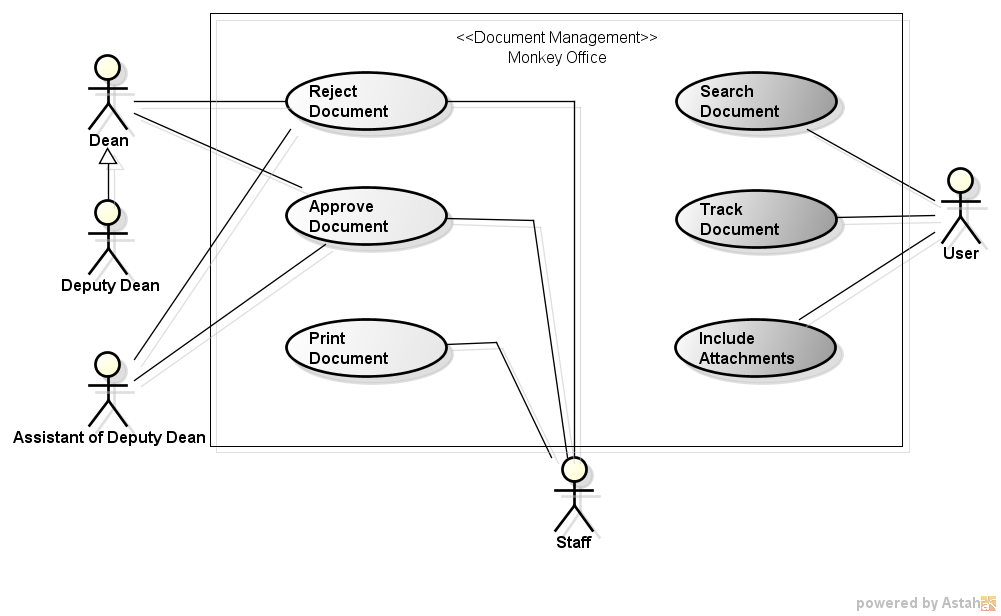
\includegraphics[scale=0.6]{res/Methodology/usecase_diagram}
	\caption{A usecase diagram for Monkey Office}
\end{figure}

\section{Storing Digital Documents}
Before storing documents, there are two things to concern.
Firstly, what metadata should be stored alongside the document so that the system can access to the digital file including its attachments.
Attachments are documents.
They can be official or unofficial documents.
Both official and unofficial documents are the same except for one characteristic.
Official documents has a customized identification code as mentioned in table \ref{tbl-doc-subtype}.
Unofficial documents has only regular identification number starting at one and increment by one for each document.
Therefore, the parent document have to store a list of attachments.
That is a list referring to itself.
A class diagram \ref{fig-doc-template} shows 
%\begin{figure*}
%	\label{fig-doc-template}
%	\caption{text}
	%\includegraphics[scale=0.5]{res/Methodology/DocumentTemplating}
%\end{figure*}

Secondly, where digital files should reside in the the server.


\section{Retrieving Digital Documents}

\section{Tracking Digital Documents}